\section{Data}
\label{sec:data}

\subsection{The POLYMOD Contact Survey}
\label{subsec:polymod_intro}
The empirical foundation of this study relies on the POLYMOD dataset, a large-scale prospective survey of social mixing patterns conducted across eight European countries \parencite{mossong2008social}.
The survey was designed to quantify the nature of social interactions relevant to the transmission of respiratory and close-contact infectious diseases.
A total of 7,290 participants recorded their daily social interactions using a standardized paper-diary methodology \parencite{mossong2008social}.

The raw dataset fundamentally consists of two levels of information: participant-level data and contact-level data.
For each recorded contact, the diaries captured detailed characteristics, including the estimated age and gender of the contacted individual, the location of the interaction, the duration and frequency of the contact, and whether physical skin-to-skin contact occurred \parencite{mossong2008social}.
This rich multidimensional data provides the essential structure required to infer human contact networks and accurately simulate epidemic dynamics.

The survey covers eight European countries: Belgium, Germany, Finland, Great Britain, Italy, Luxembourg, the Netherlands, and Poland.
Participants were recruited from a broad demographic spectrum, ensuring that the collected contact patterns represent a diverse range of socio-economic and cultural contexts.
The robustness and cross-national consistency of the mixing patterns identified in POLYMOD have been further validated by subsequent large-scale modeling efforts.
Specifically, \textcite{prem2017projecting} and \textcite{mistry2021inferring} utilized the original POLYMOD matrices to construct and project synthetic contact matrices for diverse global settings beyond the original European context.
These studies underscore that while macroscopic mixing patterns vary across countries, the setting-specific contact probabilities captured by POLYMOD remain a gold standard for projecting transmission dynamics in a global context when combined with local demographic data.

\subsection{Data Cleaning and Preprocessing}
\label{subsec:data_cleaning}
To prepare the raw diary data for computational network inference, a series of systematic data cleaning and deterministic imputation procedures were applied. 
When exact ages of contacted individuals (\texttt{cnt\_age\_exact}) were not provided, the contact age (\texttt{cnt\_age}) was estimated as the midpoint between the recorded minimum and maximum estimated ages.
If only the minimum or maximum boundary was recorded, the available boundary value was utilized.

Missing values in key categorical variables were handled deterministically based on logical baselines: missing physical contact flags were replaced with a default indicating no physical contact, while unrecorded contact frequencies and durations were imputed with the lowest respective default categories.
Furthermore, individual location flags were consolidated into a single categorical variable (\texttt{location\_category}), classifying each interaction into primary settings such as School, Work, Home, Transport, Leisure, or Other.

Because the participants represent the core vertices (nodes) of the subsequent contact network models, any participant records with missing age (\texttt{part\_age}) or gender (\texttt{part\_gender}) were strictly excluded from the dataset.
Specifically, missing values accounted for approximately 0.12\% of the contact age and 1.39\% of the contact gender across all recorded interactions.
To address this, stochastic statistical imputation was performed for these missing attributes of the contacted individuals. 
Missing contact ages were imputed by constructing a reference pool grouped by the participant's age and the contact location category.
A value was then randomly sampled from the corresponding pool's empirical distribution.
If no corresponding reference pool existed, the participant's own age was assumed.
Similarly, missing contact genders were randomly drawn based on the overall probability distribution of contact genders within the dataset.


\subsection{Exploratory Data Analysis (EDA)}
\label{subsec:eda}

Prior to the construction of generative network models, an exploratory analysis was performed on the cleaned POLYMOD dataset.
This analysis aims to identify the fundamental structural characteristics and systemic biases inherent in human social mixing.

\subsubsection{Participant Demographics}
The foundation of any contact network is the demographic composition of its constituent nodes.
Figure \ref{fig:eda_demographics} illustrates the age distribution and gender ratio of the sampled survey participants.
The gender ratio is approximately balanced, with females comprising 52.5\% of the sample.
The age distribution features a prominent concentration of individuals between 10 and 20 years old, followed by a gradual decline in older age cohorts.
These empirical attributes directly inform the nodal characteristics required for the subsequent synthetic network generation.

\begin{figure}[H]
    \centering
    \begin{minipage}{0.48\textwidth}
        \centering
        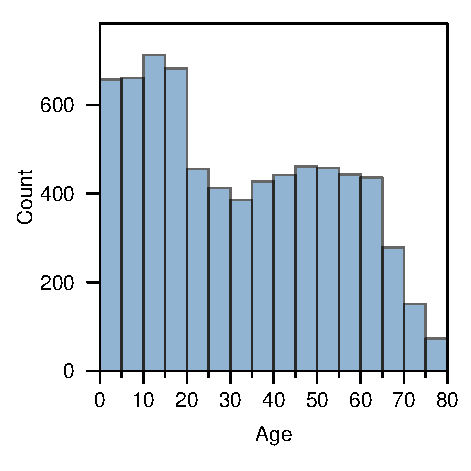
\includegraphics[width=\linewidth]{figures/02_Data/polymod_age_distribution.pdf}
    \end{minipage}\hfill
    \begin{minipage}{0.48\textwidth}
        \centering
        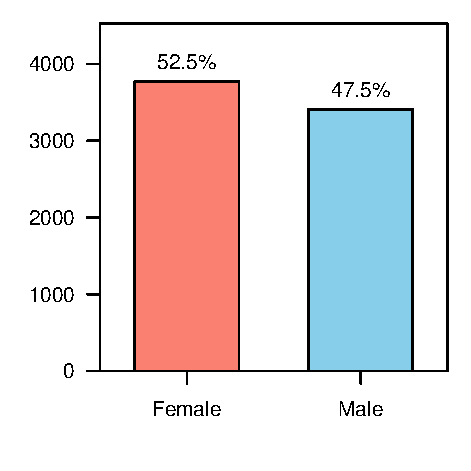
\includegraphics[width=\linewidth]{figures/02_Data/polymod_gender_ratio.pdf}
    \end{minipage}
    \caption{Participant demographics of the cleaned POLYMOD dataset. The left panel shows the age distribution with 5-year intervals, and the right panel displays the overall gender ratio.}
    \label{fig:eda_demographics}
\end{figure}

\subsubsection{Macroscopic Mixing Patterns}
Beyond individual attributes, the macroscopic volume and preference of interactions are captured by the contact matrix.
As visualized in Figure \ref{fig:eda_matrix}, the empirical data reveals a striking concentration of contacts along the main diagonal.
This intense diagonal band confirms the presence of strong age assortativity, indicating a universal human tendency to interact primarily with peers of a similar age.
Notably, the intensity of this assortative mixing is most pronounced among adolescents and young adults, reflecting the high-density contact environments characteristic of these life stages.
This concentrated activity among youths serves as a critical focal point for potential epidemic acceleration, which will be further explored in Chapter 4.

\begin{figure}[H]
    \centering
    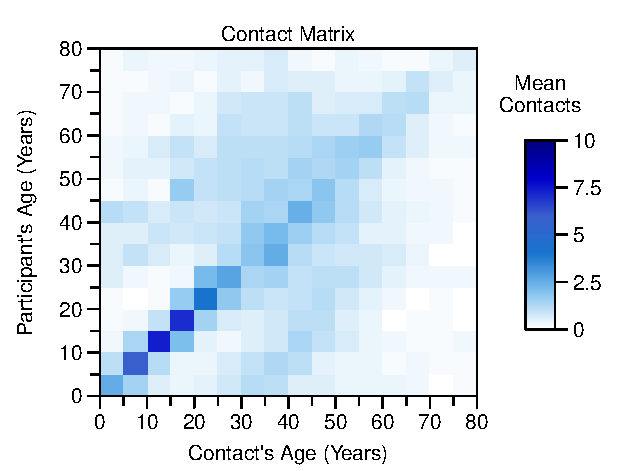
\includegraphics{figures/02_Data/polymod_contact_matrix_legend.pdf}
    \caption{Empirical contact matrix demonstrating strong age-assortative mixing. The darker blue cells along the diagonal indicate higher frequencies of interaction between individuals of the same age group.}
    \label{fig:eda_matrix}
\end{figure}

\subsubsection{Context-Specific Mixing Mechanisms}
While the macroscopic matrix highlights overall assortativity, disaggregating the contacts by location reveals distinct, context-specific mixing rules.
Figure \ref{fig:eda_location} presents the probability density of the absolute age difference between contacting pairs across four primary settings: Home, School, Work, and Leisure.
The school environment is characterized by an extreme, singular spike at an age difference of zero, demonstrating a rigid, highly stratified cohort structure.
Conversely, interactions within the home exhibit a bimodal distribution.
This bimodal shape consists of a primary peak at zero age difference, representing interactions between siblings or spouses, and a broader secondary peak around 30 years, representing inter-generational interactions between parents and children.
These empirical observations conclusively demonstrate that social networks are governed by multiple, overlapping spatial rules rather than a single homogeneous mixing parameter.
Consequently, capturing these dual mechanisms---the localized institutional clustering of schools and the broader inter-generational bridges of households---provides the foundational empirical justification for the mixture density architecture proposed in Model 2B.

\begin{figure}[H]
    \centering
    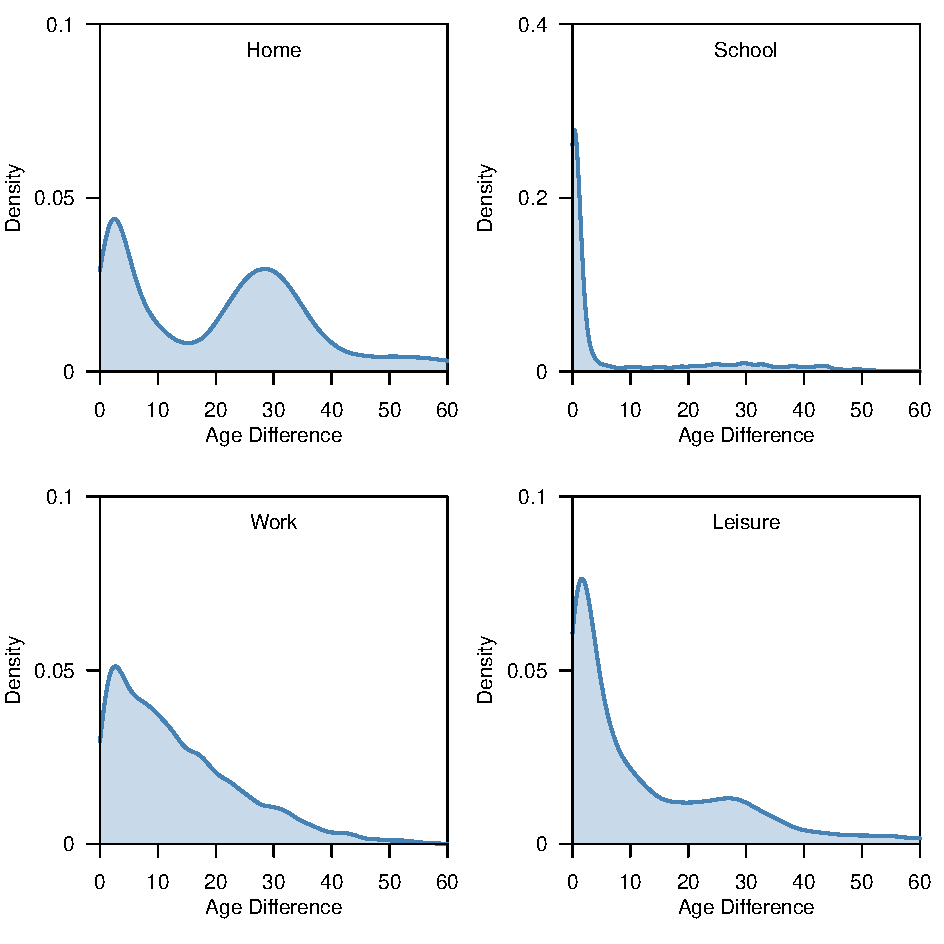
\includegraphics{figures/02_Data/polymod_agediff_location.pdf}
    \caption{Probability density of absolute age differences by contact location. The strict zero-difference spike in schools contrasts sharply with the bimodal (peer and inter-generational) distribution observed in households.}
    \label{fig:eda_location}
\end{figure}

\subsection{Population Sampling and Node Definition}
\label{subsec:sampling}
To bridge the gap between empirical data and computational simulation, we utilize a two-tier sampling strategy based on the cleaned POLYMOD distributions.
For the parameter inference stage (Section \ref{sec:inference}), a subset of $N = 1000$ unique participants was drawn using random sampling without replacement.
This reduced scale is mathematically necessary to manage the significant computational cost of the multi-stage Adaptive MCMC algorithm while preserving sufficient demographic heterogeneity.
For the subsequent large-scale epidemic simulations (Section \ref{sec:epidemic_model}), we expanded the node set to $N = 10,000$ individuals.
This larger synthetic population was sampled based on the Year 2000 European demographic distribution, ensuring that the infectious disease dynamics reflect a realistic societal scale.
Each node in these synthetic populations is assigned the age and gender attributes from the corresponding empirical records, grounding our simulations in the actual sociological landscape captured by the survey.